
\documentclass{article}


\usepackage{amsmath}
\usepackage{amssymb}
\usepackage{graphicx}

\graphicspath{ {./images/} }

\setlength{\parskip}{0.5\baselineskip plus2pt minus2pt}
\setlength\parindent{0pt}
\setlength{\textheight}{9in}

\title{WS1 Exam presentation}

\begin{document}
\section{Exercise 2}
We are now using the stochastic matrix, where we will have $t \in \mathbb{N}_0$.

\begin{equation}
    P =
    \begin{bmatrix}
    0 & 1/2 & 1/2 & 1/2 & 1/2 \\
    1/4 & 1/8 & 1/8 & 1/8 & 1/8 \\
    1/4 & 1/8 & 1/8 & 1/8 & 1/8 \\
    1/4 & 1/8 & 1/8 & 1/8 & 1/8 \\
    1/4 & 1/8 & 1/8 & 1/8 & 1/8
    \end{bmatrix}
\end{equation}

\subsection{Hvad er sandsynligheden for at v\ae re i tilstand $w_1$ til tiden $t=5$, hvis vi bruger startfordelingen fra $(1)$ og den stokastiske matrix $P$?}

\begin{equation}
    w_0 =
    \begin{bmatrix}
        1/2 \\
        1/8 \\
        1/8 \\
        1/8 \\
        1/8
    \end{bmatrix}
\end{equation}

\begin{equation}
    x_k = P^kx_0 \text{ for } k=0,1 \dots
\end{equation}

\begin{figure}[h]
    \centering
    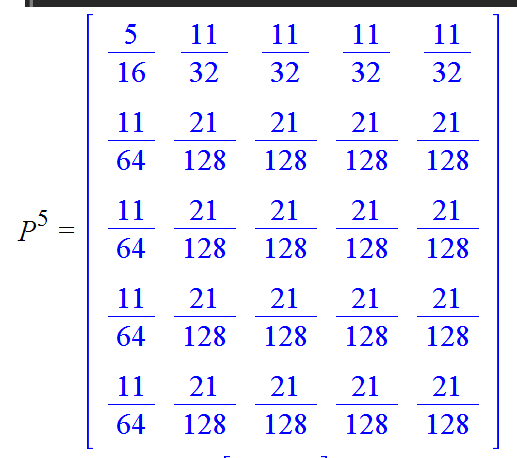
\includegraphics[width = 0.5\textwidth]{p5}
\end{figure}

\begin{equation}
    w_5 = P^5 \cdot w_0 =
    \begin{bmatrix}
        21/64 \\
        43/256 \\
        43/256 \\
        43/256 \\
        43/256 \\
    \end{bmatrix}
\end{equation}

\subsection{Har Markov-k\ae den en station\ae r fordeling? Hvis ja, bestem s\aa dan en.}

\begin{equation}
    \begin{array}{c}
        Pq = q \\
        Pq - q = 0 \\
        (P - I)q = 0
    \end{array}
\end{equation}

\begin{figure}[h]
    \centering
    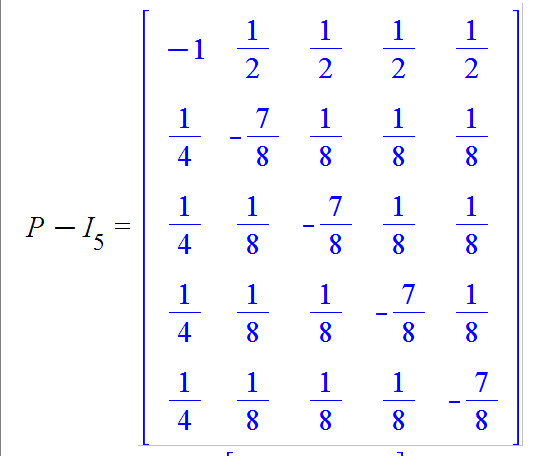
\includegraphics[width = 0.5\textwidth]{pi}
\end{figure}

\begin{figure}[h]
    \centering
    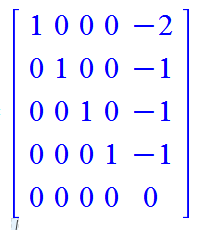
\includegraphics[width = 0.25\textwidth]{rrefpi}
\end{figure}

\begin{equation}
    v = x_5 \cdot
    \begin{bmatrix}
        2 \\
        1 \\
        1 \\
        1 \\
        1
    \end{bmatrix}
\end{equation}

\begin{equation}
    x_5(2 + 1 + 1 + 1 + 1) = 1 \implies x_5 = 1/6
\end{equation}

\begin{equation}
    q =
    \begin{bmatrix}
        1/3 \\
        1/6 \\
        1/6 \\
        1/6 \\
        1/6
    \end{bmatrix}
\end{equation}

\begin{figure}
    \centering
    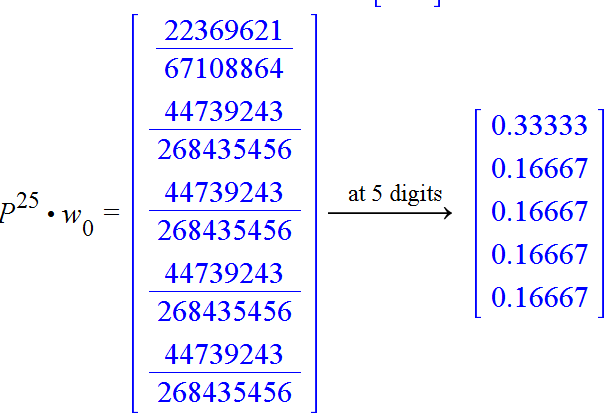
\includegraphics[width=0.5\textwidth]{check}
\end{figure}

\end{document}
